\section{Evaluation of correlation methods for co-occurrence network construction of rice crop health survey data}

\subsection*{Introduction}

Rice is not threatened by one, but by many pests in a season. A combination of injuries caused by diseases and rice pests can be thought of as a crop health syndrome. The development a crop health syndrome depend on the production situation (\textit{i.e.}, the cultural practices, inputs used to produce a rice crop) as a range of agroecosystem \citep{Savary_2006_Quantification}.

A characterization study based on survey data collected in South and South East Asia \citep{Savary_2000_Characterization} showed the patterns of crop health syndromes were common and different across sites. The study indicated that sheath blight, brown spot and leaf blast are the most important diseases and were commonly found in some sites, causing yield loss between 1 to 10%. Among insect injuries, stem borer caused yield losses of 2.3%. \citep{Savary_2000_Characterization} characterized patterns of injury profiles into five groups. For example, injury profile group1 (IN1) was characterized by comparatively high incidence of stem rot, sheath blight, plant hopper, and whorl maggot injuries, but low brown spot, and absence of bacterial leaf blight, leaf blast, and neck blast Asia.

Networks are ubiquitous systems in nature, technology and society (Newman, 2003). A network is defined as one or more sets of nodes connected by links in various ways. A node can represent the individual units depending on the context. Links or edges are the connections between nodes, which may be directed or undirected. Network models are now becoming increasingly interesting and useful in social science, biology, and ecology. The network applications  are also relevant in plant pathology were also increasingly studied \citep{Moslonka_Lefebvre_2011}. And more citation.

Network analysis is a promising tool frequently used to describe the pairwise relationships of a large number of variables. For example, association networks or correlation networks were represented by their association or correlation (adjacency) matrices, which rows and columns denote nodes, and matrix entries denote links. They were widely applied in biological studies \citep{Toubiana_2013_Net, Barabasi_2004_Network}

Selecting the most suitable correlation methods for correlation network construction is important since different correlation measures lead to different network structure and provide different information. In this chapter, four correlation methods, including Pearson, Spearman rank correlation, Kendall correlation \citep{Prokhorov_2001_Kendall} and Biweight mid-correlation, to associate rice injuries. \todo{Search for the citation of correlation.}
 

\subsection*{Materials and methods}

The method for evaluating and selecting correlation methods to construct correlation network of rice injuries in crop health survey data was showed in Fig. Finally, correlation metrics were used for the network analysis in next chapter.

\begin{figure}
    \centering
     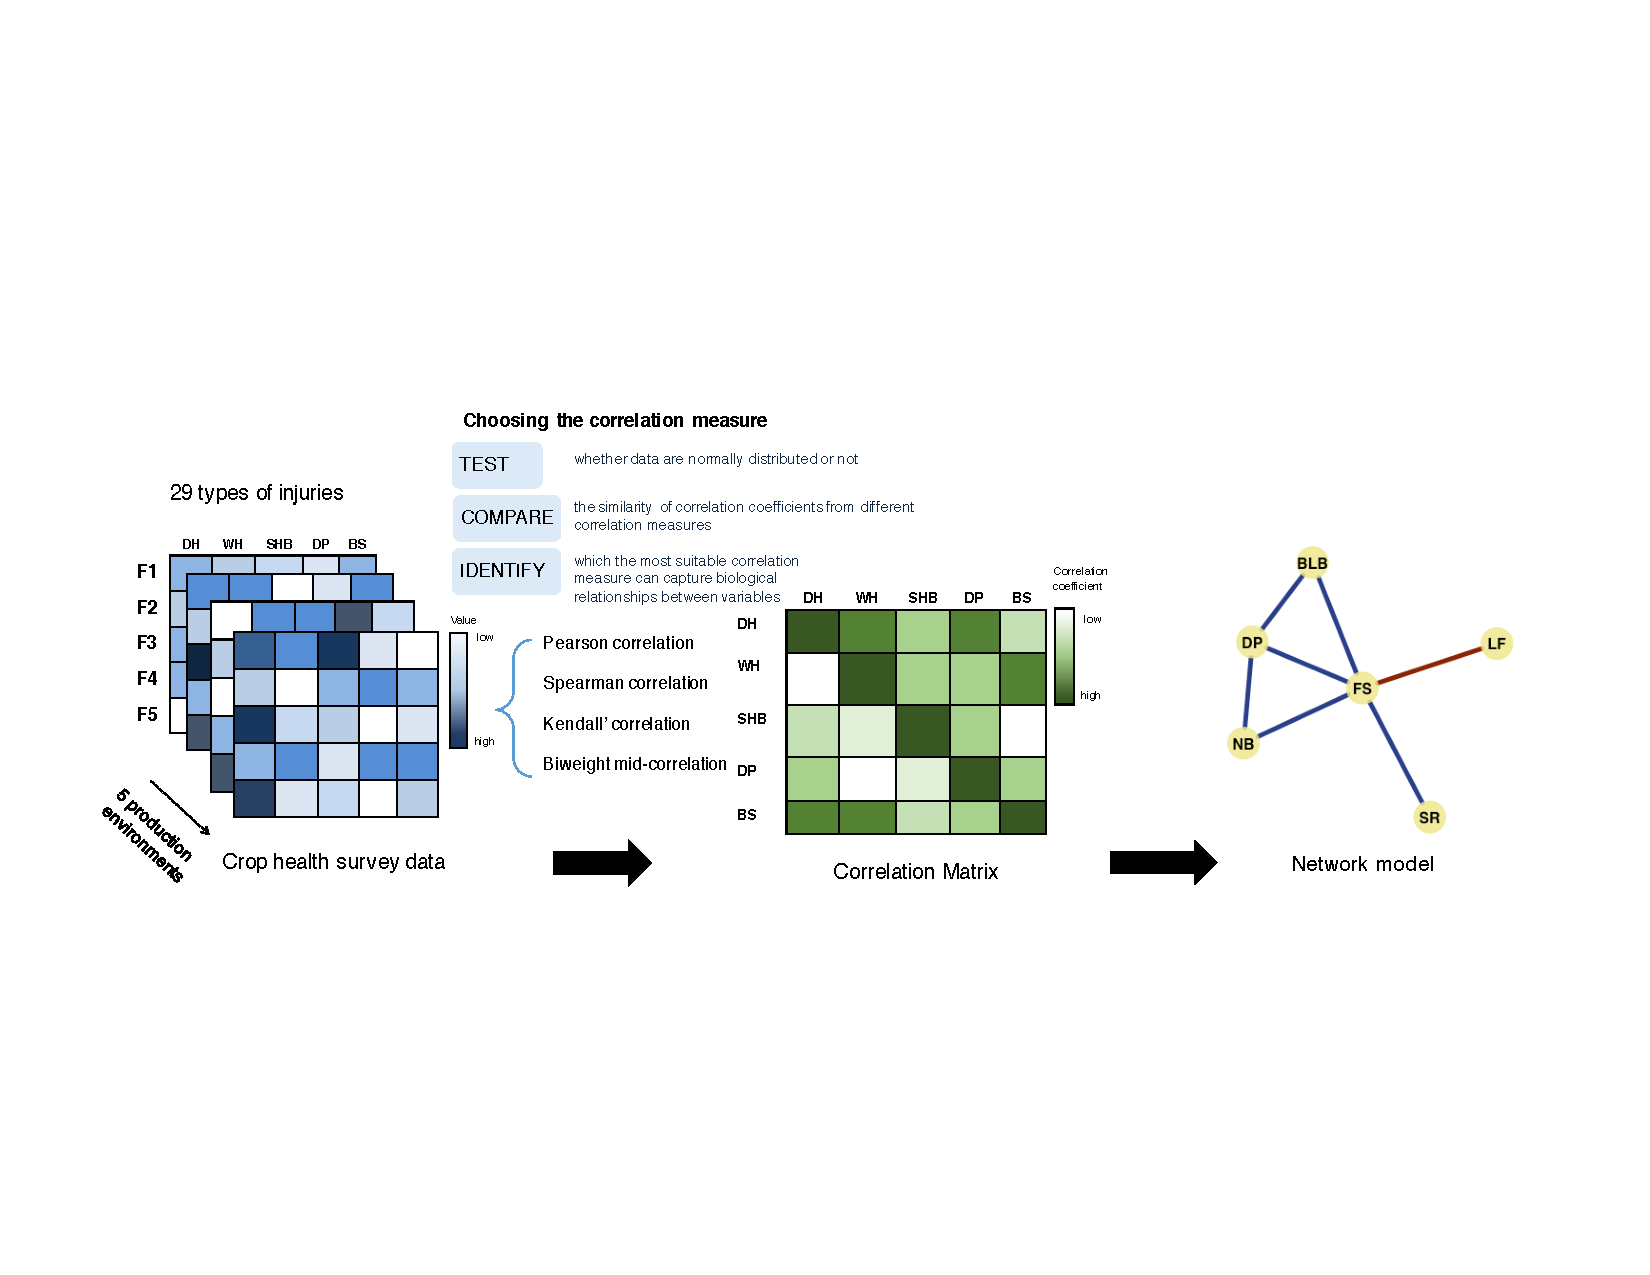
\includegraphics[width = 1\textwidth]{figures/pipeline4/pipeline4.pdf}
    \caption{Correlation methods selected for constructing network model. The plots on the left show sample survey data taken over 29 rice injuries at 5 production environments. The next step is to compute pair-wise correlations to obtain a cross-correlation matrix (the middle plot, rows and columns represent the nodes). Then, the matrix will be used for network analysis.}
    \label{fig:pipeline1}
\end{figure}

\textbf{Survey data}

Survey data was collected from 450 farmers’ fields growing rice on irrigated lowland areas across South and Southeast Asia Tamil Nadu, India (TM); Odisha, India, West Java; Indonesia; Central Plain, Thailand, and Red River Delta, Vietnam were collected from 2013 to 2016. The number of survey are summarized in Table \ref{table:Survey_data}.

% Please add the following required packages to your document preamble:
\begin{table}[]
\centering
\begin{tabular}{llllllll}
\hline
\multirow{3}{*}{Country} & \multicolumn{6}{c}{year} & \multirow{3}{*}{Total} \\ \cline{2-7}
                         & \multicolumn{2}{c}{2010} & \multicolumn{2}{c}{2011} & \multicolumn{2}{c}{2012} &                        \\ \cline{2-7}
                         & DS         & WS          & DS          & WS         & DS          & WS         &                        \\
\hline
India                    &            & 25          & 60          &            & 20          &            & 105                    \\
Indonesia                & 5          & 20          & 30          & 30         & 20          &            & 105                    \\
Philippines              &            & 20          & 20          &            &             &            & 40                     \\
Thailand                 &            & 20          &             & 45         &             & 40         & 105                    \\
Vietnam                  &            & 20          &             & 15         & 25          &            & 70                     \\
\hline
Total                    & 5          & 115         & 110         & 90         & 65          & 40         & 425    \\
\hline               
\end{tabular}
\caption{Number of farmers' fields surveyed by country and year}
\label{table:Survey_data}
\end{table}

The survey procedure and data were based on a standardized protocol described in ``A survey portfolio to characterize yield-reducing factors in rice'' developed by \citet{Savary_2009_Survey}. Twenty-nine rice injuries were collected 
including the injuries caused by animal pests, and pathogens, which are harmful to rice plants, and importantly considered to reduce yield productivity. The injuries were evaluated at booting and ripening stage according to survey procedure. They were found on different organs of rice plants depending on their natures. 

Injuries on leaves such as whorl maggot injury (WM), leaffolder injury (LF), bacterial leaf blight (BLB), bacterial leaf streak (BLS), leaf blast (LB), brown spot (BS), leaf miner injuries (LM), leaf scald (LS), narrow brown spot (NBS), rice hispa injury (RH), red stripe (RS), rice thrip injury (RTH) were determined as a proportion of injured leaves. Injuries on tillers or hills such as stem rot (SR), sheath rot (SHR), sheath blight (SHB), whitehead (WH), deadheart (DH), silver shoot (SS), false smut (FS), Neck blast (NB), Panicle mite injury (PM), Rice bug injury (RB), rat injury (RT) were determined as a proportion of injured tillers or panicles. Systemic injuries such as Bug burn (BB), grassy stunt (GS), hopper burn( HB)  , ragged stunt (RGS), tungo (RTG) were determined as the percentage of area affected. The rice injury lists are showed in Table \ref{table:variable_des}.

\begin{table}[]
\centering
\caption{My caption}
\label{my-label}
\begin{tabular}{llll}
Injuries              & Acronym & Description1                                                                              & Unit2  \\
Deadheard             & DH      & maximum percentage of tillers with deadheart                                              & \%     \\
Whitehead             & WH      & maximum percentage of panicles with whitehead                                             & \%     \\
Silver shoot          & SS      & maximum percentage of tillers with silvershoot                                            & \%     \\
Whorl maggot          & WM      & area under the progress curve of the mean percentage of leaves with whorl maggot injury   & \% dsu \\
Leaffolder            & LF      & area under the progress curve of the mean percentage of leaves with leaffolder injury     & \% dsu \\
Leafminer             & LM      & area under the progress curve of the mean percentage of leaves with leaf miner injury     & \% dsu \\
Rice hispa            & RH      & area under the progress curve of the mean percentage of leaves with rice hispa injury     & \% dsu \\
Rice thrip            & THR     & area under the progress curve of the mean percentage of leaves with rice thrip injury     & \% dsu \\
Panicle mite          & PM      & maximum percentage of tillers with panicle mite injury                                    & \%     \\
rice bug injury       & RBP     & maximum percentage of panicles with rice bug injury                                       & \%     \\
Hopper burn           & HB      & maximum percentage of hopperburn in a one-sqm area                                        & \%     \\
Bug burn              & BB      & maximum percentage of bugburn in a one-sqm area                                           & \%     \\
Bacterial leaf blight & BLB     & area under the progress curve of the mean percentage of leaves with bacterial leaf blight & \% dsu \\
leaf blast            & LB      & area under the progress curve of the mean percentage of leaves with leaf blast            & \% dsu \\
brown spot            & BS      & area under the progress curve of the mean percentage of leaves with brown spot            & \% dsu \\
Bacterial leaf streak & BLS     & area under the progress curve of the mean percentage of leaves with bacterial leaf streak & \% dsu \\
Narrow brown spot     & NBS     & area under the progress curve of the mean percentage of leaves with narrow brown spot     & \% dsu \\
Red stripe            & RS      & area under the progress curve of mean percentage of leaves with red stripe                & \% dsu \\
Leaf scald            & LS      & area under the progress curve of mean percentage of leaves with leaf scald                & \% dsu \\
Sheath blight         & SHB     & maximum percentage of tillers with sheath blight                                          & \%     \\
Sheath rot            & SHR     & maximum percentage of tillers with sheath rot                                             & \%     \\
Stem rot              & SR      & maximum percentage of tillers with stem rot                                               & \%     \\
False smut            & FSM     & maximum percentage of panicles with false smut                                            & \%     \\
Neck blast            & NB      & maximum percentage of panicles with neck blast                                            & \%     \\
Dirty panicle         & DP      & maximum percentage of panicles with dirty panicle                                         & \%     \\
Rice tungro disease   & RTD     & maximum percentage of tungro in a one-sqm area                                            & \%     \\
Ragged stunt disease  & RSD     & maximum percentage of ragged stunt disease in a one-sqm area                              & \%     \\
gressy stunt disease  & GSD     & maximum percentage of grassy stunt disease in a one-sqm area                              & \%     \\
Rat damage            & RT      & maximum percentage of tillers with rat injury                                             & \%    
\end{tabular}
\end{table}

Before analysis, data were compacted over time during crop growth. Two types of data were computed, depending on the natures of injuries as defined by \citep{Savary_2009_Survey}. One is an area under injury progress curve (AUIPC) used for injury variables, which present on the leaves, and for weed infestation. Another is the maximum level at any of the two observations used for injury variables that can be observed on tillers, panicles, and hills, and insect pest count. The area under injury progress curve (AUIPC) \citep{Campbell_1990_Introduction} were calculated by the mid-point method using the following equation:  

\begin{equation}
AUIPC = \sum{\frac{1}{2(X_{i} + X_{i-1})(T_{i} - T_{i-1})}}
\end{equation}

where $X_i$ is percentage (\%) of leaves, tillers or panicles injured due to rice pests (e.g., leaf blast, leaf folder), or number of insects (e.g., plant hoppers, leaf hoppers) per quadrat, or percentage (\%) of weed infestation (ground coverage) at the $i$th observation, $T_i$ is time in rice development stage units (dsu) on a 0 to 100 scale (10: seedling, 20: tillering, 30: stem elongation, 40: booting, 50: heading, 60: flowering, 70: milk, 80: dough, 90: ripening, 100: fully mature) at the $i$th observation and $n$ is total number of observations.

\text{Evaluation}
In this study, correlation measures including, Pearson, Spearman, Kendal and Biweight mid-correlation \citep{Wilcox_2012_Introduction} were evaluated to discover the true functionally related variables in crop health survey data. The data will have to follow the assumption of correlation measures. The correlation measures will also be able to effectively capture biological relationships that are well published. I proposed three steps for correlation methods selection: 

\begin{itemize}
\item \textbf{Testing} whether or not the data are normally distributed by visual assessments and statistical tests. The distribution of values of rice injuries in crop health survey data was examined and tested the hypothesis hypothesis that the sample comes from a population which has a normal distribution by performed Shapiro-Wilk test.
\item \textbf{Comparing} correlation measures by testing similarity of correlation coefficients. I evaluated the similarity of correlation coefficients of different correlation measures by using the Euclidean distance, and perform clustering analysis.
\item \textbf{Identifying} the most suitable correlation measure that can capture biological relationships between variables confirm with the published relationships.
\end{itemize}

\subsection*{Result}

\textbf{Checking and testing the distribution of crop health survey data}

To determine normality of the survey data, I presented the histograms (Fig \ref{fig:allhisto}) showing distribution of value of rice injuries, calculated summary statistics, and performed Shapiro-Wilk test. The histograms depict the distribution of values of injuries. The histograms showed that values of injuries are skewed to the left. Common values of the injuries were 0. A few farmers’ fields presenting in high values of injuries were relatively low. The distribution of most injuries are described power low or long tails. ?? the power low or long tailed.

\begin{landscape}
\begin{figure}[!h]
\centering
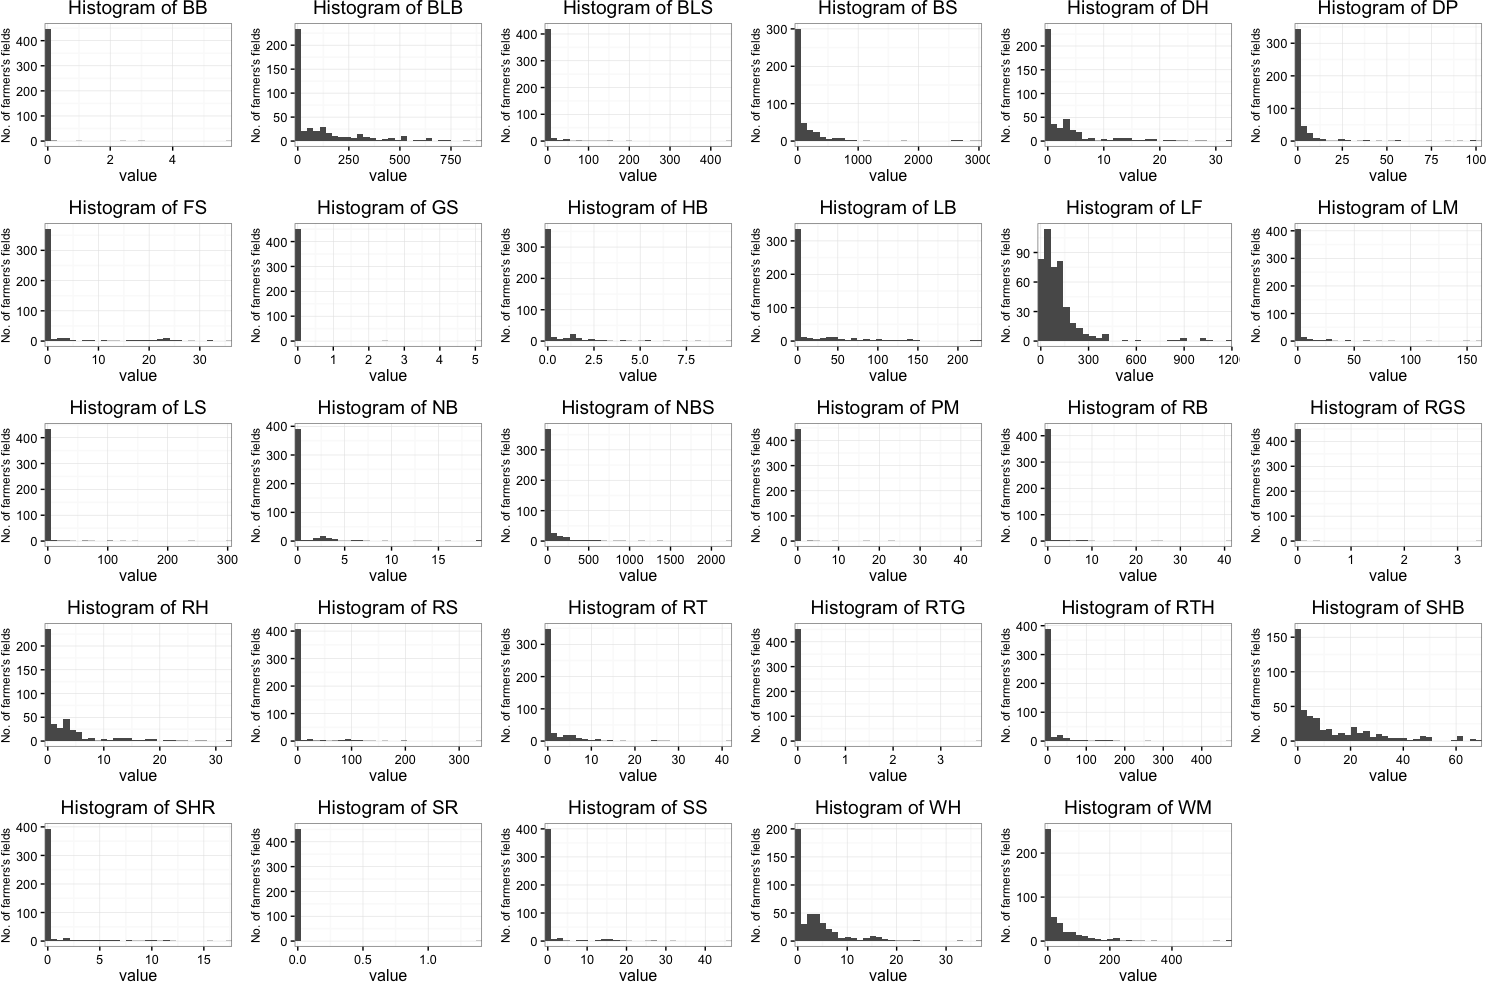
\includegraphics[width = 1\textwidth]{figures/allhisto2/allhisto2.png}
\caption{Histograms showing the distribution of rice injury values in crop health survey data. BB:Bug burn, BLB:Bacterial leaf blight, BLS: Bacterial leaf streak, BS:Brown spot, DH:Deadheart, DP: Dirty panicle, FS:False smut, GS:Gressy stunt, HB:Hopper burn, LB: Leaf blast, LF: Leaffolder injury, LM: Leaf miner injury, LS: :Leaf scald, NB:Neck blast, NBS:Nerrow brown spot, PM: Panicle mite injury, RB: Rice bug injuries, RGS:Ragged stunt, RH:Rice hispa injury, RS: Red stripe, RT:Rat damage, RTG: Tungro, RTH:Rice thrip injury, SHB:Sheath blight, SHR:Sheath rot, SNL:Snail damage, SR:Stem rot, SS:Silver shoot, WH:White head, WM:Whorl maggot injury.}
\label{fig:allhisto}
\end{figure}
\end{landscape}

\begin{landscape}
\begin{table}[]
\centering
\caption{Summary statistics of rice injuries in crop health survey data}
\begin{threeparttable}
\label{table:summary_injuries}
\begin{tabular}{lllllllllc}
\hline
Injuries & Mean   & SD\textsuperscript{1}     & Median & Min  & Max     & Skewness & Kurtosis & SE\textsuperscript{2}    & Shapiro-Wilk test\textsuperscript{3} \\
\hline
BB   & 0.03   & 0.33   & 0.00   & 0.00 & 5.80    & 14.43    & 228.44   & 0.02  & **               \\
BLB  & 113.64 & 178.34 & 0.00   & 0.00 & 886.67  & 1.86     & 2.93     & 8.38  & **               \\
BLS  & 4.94   & 28.26  & 0.00   & 0.00 & 444.48  & 10.35    & 138.48   & 1.33  & **               \\
BS   & 147.54 & 386.19 & 0.00   & 0.00 & 2999.42 & 5.09     & 30.22    & 18.14 & **               \\
DH   & 3.18   & 5.62   & 0.00   & 0.00 & 32.33   & 2.49     & 6.50     & 0.26  & **               \\
DP   & 3.54   & 12.39  & 0.00   & 0.00 & 101.62  & 5.70     & 36.17    & 0.58  & **               \\
FS   & 2.41   & 6.61   & 0.00   & 0.00 & 35.74   & 2.90     & 7.35     & 0.31  & **               \\
GS   & 0.02   & 0.26   & 0.00   & 0.00 & 5.10    & 17.38    & 317.16   & 0.01  & **               \\
HB   & 0.41   & 1.13   & 0.00   & 0.00 & 9.80    & 4.18     & 22.02    & 0.05  & **               \\
LB   & 17.06  & 38.50  & 0.00   & 0.00 & 226.21  & 2.79     & 8.43     & 1.81  & **               \\
LF   & 114.48 & 156.86 & 76.74  & 0.00 & 1180.29 & 3.94     & 18.95    & 7.37  & **               \\
LM   & 2.93   & 14.33  & 0.00   & 0.00 & 160.47  & 7.63     & 68.27    & 0.67  & **               \\
LS   & 3.13   & 22.06  & 0.00   & 0.00 & 302.08  & 9.82     & 110.91   & 1.04  & **               \\
NB   & 0.60   & 2.14   & 0.00   & 0.00 & 19.32   & 5.69     & 38.72    & 0.10  & **               \\
NBS  & 53.98  & 178.50 & 0.00   & 0.00 & 2213.54 & 6.49     & 58.95    & 8.39  & **               \\
PM   & 0.23   & 2.51   & 0.00   & 0.00 & 44.42   & 14.35    & 229.31   & 0.12  & **               \\
RB   & 0.53   & 3.08   & 0.00   & 0.00 & 40.98   & 8.52     & 87.20    & 0.14  & **               \\
RGS  & 0.01   & 0.16   & 0.00   & 0.00 & 3.40    & 21.02    & 445.24   & 0.01  & **               \\
RH   & 3.18   & 5.62   & 0.00   & 0.00 & 32.33   & 2.49     & 6.50     & 0.26  & **               \\
RS   & 8.14   & 31.13  & 0.00   & 0.00 & 336.71  & 5.32     & 37.10    & 1.46  & **               \\
RT   & 1.47   & 4.02   & 0.00   & 0.00 & 41.56   & 4.90     & 32.92    & 0.19  & **               \\
RTG  & 0.01   & 0.18   & 0.00   & 0.00 & 3.80    & 21.28    & 453.00   & 0.01  & **               \\
RTH  & 9.01   & 34.69  & 0.00   & 0.00 & 470.55  & 7.52     & 79.09    & 1.63  & **               \\
SHB  & 11.67  & 15.49  & 4.72   & 0.00 & 68.65   & 1.60     & 2.08     & 0.73  & **               \\
SHR  & 0.66   & 2.23   & 0.00   & 0.00 & 17.41   & 4.24     & 19.76    & 0.10  & **               \\
SR   & 0.00   & 0.07   & 0.00   & 0.00 & 1.39    & 21.28    & 453.00   & 0.00  & **               \\
SS   & 1.40   & 4.91   & 0.00   & 0.00 & 46.01   & 4.47     & 24.33    & 0.23  & **               \\
WH   & 3.53   & 5.18   & 1.67   & 0.00 & 36.64   & 2.36     & 7.45     & 0.24  & **               \\
WM   & 36.72  & 71.63  & 0.00   & 0.00 & 583.41  & 3.84     & 21.16    & 3.37  & **               \\ 
\hline
\end{tabular}
\begin{tablenotes}
     \item[1]Stardard variation \\
     \item[2]Standard Error \\
     \item[3]** is significant at $p$ < 0.01
\end{tablenotes}
\end{threeparttable}
\end{table}
\end{landscape}

The summary statistics, and the result of Shapiro-Wick test of each injury were calculated and summarized in Table \ref{table:summary_injuries}.  As can be seen, from the previous observations that rice injuries histograms tend to be positively skewed, the median values of injuries were considered due to their insensitivity to outliers. Median of injuries were almost 0, except LF. According to \citet{Doane_2011_Measuring}, skewness and kurtosis values were more than 0, which mean that the values of injuries were asymmetrically distributed with a long tail to the right. The normality is defined as $p$ value 0.01 in Shapiro-Wilk testing. That test indicates that values of injuries were not normally distributed.

\textbf{Comparing correlation coefficients of rice injuries from four correlation methods }

I performed pair-wise analysis between each of injuries using all four correlation methods (Pearson, Spearman, Kendall correlation, and Biweight mid-correlation). I examined the similarity of correlation coefficients and clustered according to hierarchical clustering using Euclidean distance. The result is shown in Figure \ref{fig:heatmap}. Two groups of correlation methods can be distinguished: (i) parametric correlation measures (Pearson correlation and Biweight mid-correlation) and (ii) nonparametric correlation measure (Spearman correlation and Kendall correlation).
\begin{figure}[!h]
\centering
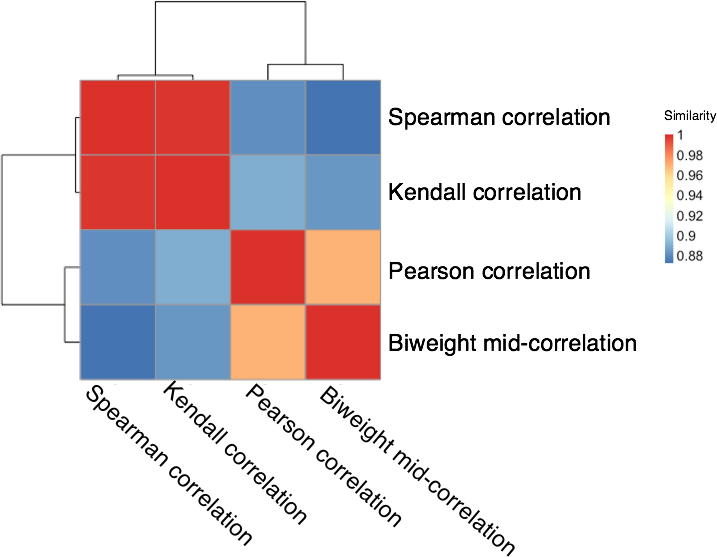
\includegraphics[width = 1\textwidth]{figures/heatmap/heatmap.png}
\caption{Heatmap and dendrogram showing hierarchical unsupervised clustering analysis correlation measures of survey data}
\label{fig:heatmap}
\end{figure}

\textbf{Identify the most suitable correlation measure}
% not clear give more explaination
% show the examples that Spearmen show better than Kendall

Although examination of correlation coefficients from correlation methods, it was also interested in learning the efficiency of each method if the output of each method were cut off by a threshold $p$-value. Since the resultant $p$-values from different methods can be different, I obtain the a higher number of significant injury pairs and a small number of significant injury pairs when implementing the same cut-off $p$-value threshold (e.g. $p$-value, 0.05) on different methods, making it difficult to compare the efficiency of different methods (see Table \ref{table:allhisto}). Outputs for each method was sorted by $p$-values in ascending order and cut off at $p$-value < 0.05.  Spearman method could capture 182 pairwise relationships, following with Biweight-mid correlation Pearson method captures and Kendall with respectively, which could captured 120, 126, and 86 significant pairwise relationships. In a series of different cut-off $p$-values, it was generally high number of injury pairs resulting from Spearman appeared to be higher than Biweight, Pearson, and Kendall.

According to the previous results, the group of parametric correlation measures was selected out because these measures required the data normally distributed. So I would consider the correlation measures in the group of rank based methods that do not required normality. Compared between Spearman and Kendall correlation, the pair-wise relationships of rice injuries were captured differently. One of many relationships captured by Spearman correlation method,but not by Kendall methods is dirty panicle – brown spot relationship (Table). This relationship has been reported in many studies \citep{Ou_1985_Rice, Barnwal_2013_Review}.

\subsection{Discussion}

An important criteria to select the suitable correlation measures is to check normality of the variables analysed, because a vital assumption in Pearson’s contribution is the normality of the variables analysed, which could be true only for quantitative variables. Pearson’s correlation coefficient is a measure of the strength of the linear relationship between two such variables. Thus, it is worth to check and test this assumption. Based on visual assessment of the histograms, all the variables show a skewness to the left skewed clearly. Skewness and kurtosis values were higher than zero, which indicated that the populations were not non-normal distribution  according to \citet{Doane_2011_Measuring}. Visual inspection of the distribution may be used for assessing normality, although this approach is usually unreliable and does not guarantee that the distribution is normal \citep{Ghasemi_2012_Normality}. So normality tests were suggested such as Kolmogorov-Smirnov test, Shapiro-Wilk test. Some researchers recommend the Shapiro-Wilk test as the best choice for testing the normality of data \citep{Peat_2005_Guide}. Shapiro-Wilk test showed that these results were in accord with skewness and kurtosis values.

Evaluation of four correlation measures, including Pearson, Spearman, Kendall correlation, and Biweight mid-correlation by determining similarity of correlation coefficients from each method. The results showed two groups clustered according to hierarchical clustering using Euclidean distance. The Spearman and Kendall correlation were grouped in rank-base methods, and another group is non-rank-based correlations including Pearson correlation and Biweight mid-correlation. From the previous result of testing normality of data, it suggested that the data did not meet the assumption of parametric correlation methods, such as Pearson' method. However, Pearson correlation coefficient is sensitive to outliers (citation). Biweight midcorrelation is considered to be a good alternative to Pearson correlation since it is more robust to outliers\citep{Wilcox_2012_Introduction}. Among the four correlation methods, Spearman and Kendall are nonparametric rank-based methods. The rank-base methods are nonparametric (distribution-free) statistics, which uses ranks for correlation and therefore provides a robust measure of a monotonic relationship between two continuous random variables. For this reason, they are particularly suitable for identifying the injuries that increase or decline in monotonic trends in survey data collected during a biological processes or developmental stages.

% review and revised it is unclear 
Although we can opt for a method based on its principle of statistical operation without paying attention to the biological models in a given data set, this may not lead to a coordination network that will reveal biological knowledge \citep{Kumari_2012_Evaluation}. The appropriate correlation measures for studied data should closely associate to the prior knowledge of biological correlation. For this study, relationship between dirty panicle and brow spot was detected by Spearman correlation but not by other correlation methods.

\subsection{Conclusions}

The analyses I have performed clearly demonstrate the distinct and common performance of four correlation methods. Pearson has been widely used in correlation analyses \citep{Zhang_2005_General}. However, Pearson correlation is limited to be suitable to normally distributed data, and is only able to capture the linear relationships. Biweight mid-correlation is more robust to  take outlier  into account compared to Pearson method, but this is not seem relevant for this survey data, as the outputs between the two methods were not different (in same cluster). The Spearman and Kendall method performed ?? and can capture many relationships in this survey data. Chosen between these methods, Spearman could capture and identify biologically or functionally associated injuries.

The Pearson and Distance Covariance methods are distinct and generally are less valuable for identifying biologically or functionally associated genes. Unfortunately, the efficiency of different methods indeed varies with the biological processes.